\chapter{Планиметрия: треугольники, окружности и площади}\label{chap:plane-geometry}\markright{Глава 28}

\section{Фигуры, расстояния и углы}
\begin{definition}\term{Планиметрия} (\emph{plane geometry}) изучает фигуры евклидовой плоскости. Точки и прямые принимаются как исходные объекты. Через две различные точки проходит ровно одна прямая; через точку вне прямой проходит ровно одна параллельная ей прямая.\end{definition}
\begin{definition}\term{Отрезок} (\emph{line segment}) \(AB\) — часть прямой между \(A,B\), включая концы. Его длина обозначается \(|AB|\) или \(AB\), когда речь идёт о числе.\end{definition}
\begin{definition}\term{Угол} (\emph{angle}) образован двумя лучами с общим началом. Развёрнутый угол равен \(\pi\) радиан, или \(180^\circ\); прямой — \(\frac\pi2\), или \(90^\circ\).\end{definition}
\begin{definition}\term{Параллельные прямые} (\emph{parallel lines}) лежат в одной плоскости и не пересекаются. \par\term{Перпендикулярные прямые} (\emph{perpendicular lines}) пересекаются под прямым углом.\end{definition}
\par\addvspace{5pt}\begin{lrbox}{\CatFlowBox}\begin{minipage}[t]{\linewidth}
\setlength{\parskip}{5pt}\setlength{\columnsep}{4.5mm}\setlength{\intextsep}{0pt}
\begin{wrapfigure}[9]{r}{54mm}
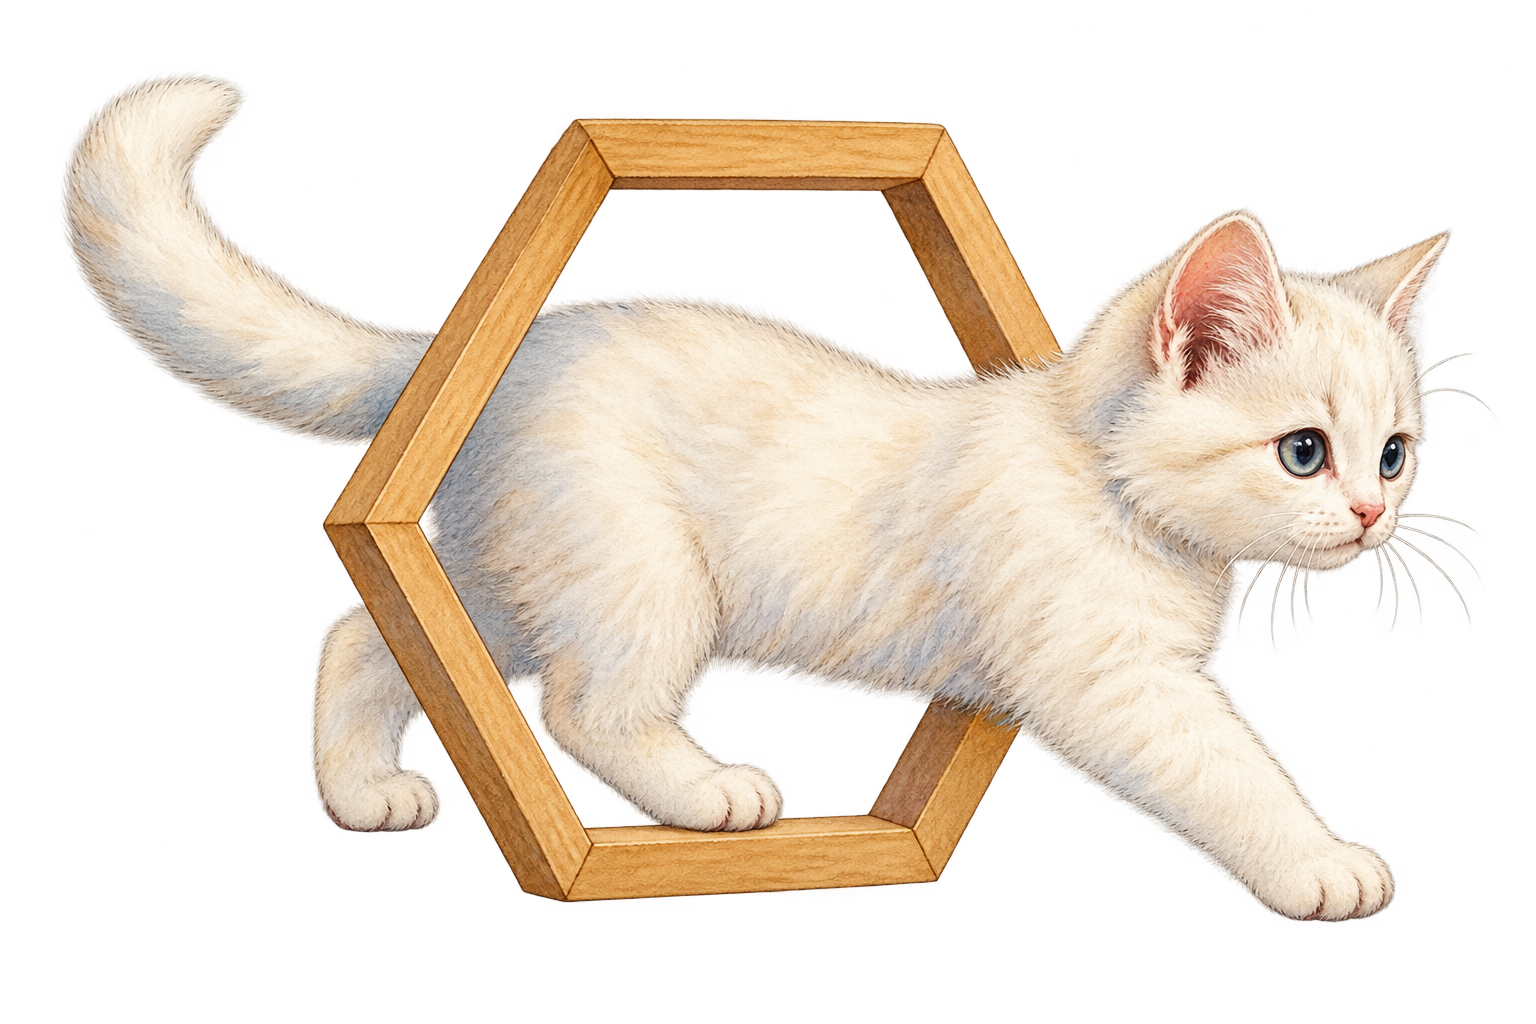
\includegraphics[width=54mm,height=58mm,keepaspectratio]{images/unique/art-136.png}
\label{catflow:136}
\end{wrapfigure}
Чертёж помогает обнаружить соотношение, но сам по себе не доказывает его. Две линии могут казаться перпендикулярными из-за масштаба рисунка. В доказательстве нужны условия задачи, определения и уже установленные свойства. Численные подписи на рисунке считаются данными только тогда, когда они указаны в условии.
\par\WFclear\end{minipage}\end{lrbox}%
\ifdim\dimexpr\ht\CatFlowBox+\dp\CatFlowBox\relax<64mm\dp\CatFlowBox=\dimexpr64mm-\ht\CatFlowBox\relax\fi%
\noindent\usebox{\CatFlowBox}\par\addvspace{5pt}
\begin{definition}\term{Треугольник} (\emph{triangle}) — фигура с тремя не лежащими на одной прямой вершинами и соединяющими их сторонами. Стороны \(a,b,c\) лежат напротив углов \(A,B,C\). Для невырожденного треугольника каждая сторона строго меньше суммы двух других.\end{definition}
\begin{theorem}[Сумма углов треугольника]
\(A+B+C=\pi\). Внешний угол равен сумме двух внутренних углов, не смежных с ним.
\end{theorem}
\begin{proof}Проведём через одну вершину прямую, параллельную противоположной стороне. Накрест лежащие углы равны, поэтому три внутренних угла составляют развёрнутый угол. Для внешнего угла вычитаем смежный внутренний из \(\pi\).\end{proof}
\begin{definition}\term{Равные треугольники} (\emph{congruent triangles}) совмещаются движением плоскости; соответствующие длины и углы совпадают. Стандартные признаки равенства: по трём сторонам; по двум сторонам и углу между ними; по стороне и двум прилежащим углам. Они выражают однозначность построения треугольника с такими данными.\end{definition}
\begin{definition}\term{Медиана} (\emph{median}) соединяет вершину с серединой противоположной стороны.\end{definition}
\begin{definition}\term{Биссектриса} (\emph{angle bisector}) делит угол на два равных угла.\end{definition}
\begin{definition}\term{Высота треугольника} (\emph{altitude}) — перпендикуляр из вершины к прямой, содержащей противоположную сторону. У тупоугольного треугольника основание высоты может лежать на продолжении стороны.\end{definition}
\section{Подобие и масштаб}
\begin{definition}\term{Подобные треугольники} (\emph{similar triangles}) имеют равные соответствующие углы и пропорциональные соответствующие стороны. Общий положительный множитель длин называется коэффициентом подобия.\end{definition}
\begin{theorem}[Подобие по двум углам]
Равенство двух соответствующих углов двух треугольников влечёт их подобие.
\end{theorem}
\begin{proof}Совместим одну вершину и один исходящий из неё луч движением плоскости. Растяжением с центром в этой вершине совместим конец первой стороны. Растяжение умножает все длины на один положительный коэффициент и сохраняет углы. Второй луч из первой вершины и луч из второй вершины определены заданными углами; их единственное пересечение задаёт третью вершину. После растяжения треугольники совпали.\end{proof}
\par\addvspace{5pt}\begin{lrbox}{\CatFlowBox}\begin{minipage}[t]{\linewidth}
\setlength{\parskip}{5pt}\setlength{\columnsep}{4.5mm}\setlength{\intextsep}{0pt}
\begin{wrapfigure}[10]{l}{54mm}
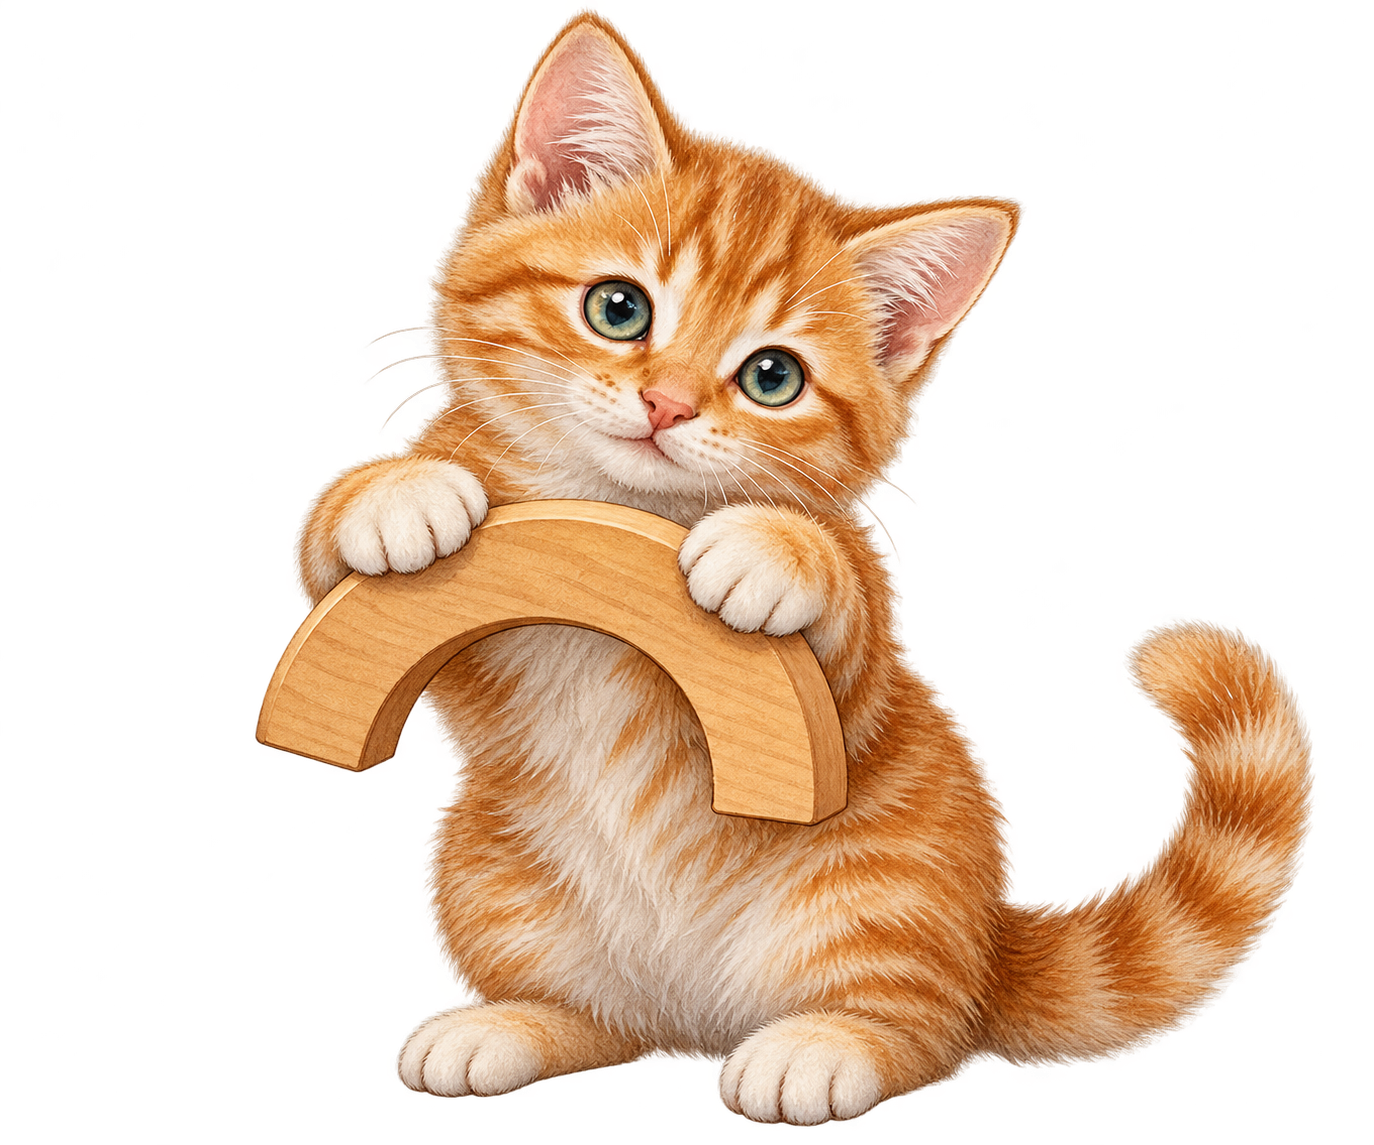
\includegraphics[width=54mm,height=58mm,keepaspectratio]{images/unique/art-137.png}
\label{catflow:137}
\end{wrapfigure}
При увеличении чертежа в \(k>0\) раз длины умножаются на \(k\), а площади — на \(k^2\). Например, план комнаты в масштабе \(1:100\) уменьшает длины в сто раз, но площади в десять тысяч раз. Это различие важно и при сравнении подобных треугольников, и при пересчёте единиц площади.
\par\WFclear\end{minipage}\end{lrbox}%
\ifdim\dimexpr\ht\CatFlowBox+\dp\CatFlowBox\relax<64mm\dp\CatFlowBox=\dimexpr64mm-\ht\CatFlowBox\relax\fi%
\noindent\usebox{\CatFlowBox}\par\addvspace{5pt}
\begin{theorem}[Параллельное сечение треугольника]
Если \(D\in AB\), \(E\in AC\) и \(DE\parallel BC\), то
\[
\frac{AD}{AB}=\frac{AE}{AC}=\frac{DE}{BC}.
\]
\end{theorem}
\begin{proof}У треугольников \(ADE,ABC\) общий угол при \(A\), а соответствующие углы при \(D,B\) равны из-за параллельности. Применяем подобие по двум углам.\end{proof}
\section{Окружность, касательная и степень точки}
\begin{definition}\term{Окружность} (\emph{circle}) с центром \(O\) и радиусом \(R>0\) состоит из точек на расстоянии \(R\) от \(O\). \par\term{Круг} (\emph{disk}) включает и внутренние точки: \(OP\le R\).\end{definition}
\begin{definition}\term{Описанная окружность треугольника} (\emph{circumcircle}) проходит через все его вершины. Её центр — пересечение серединных перпендикуляров к сторонам: каждая такая прямая задаёт равноудалённость от двух вершин. Две прямые пересекаются в единственной точке, поскольку вершины не лежат на одной прямой.\end{definition}
\begin{definition}\term{Хорда} (\emph{chord}) соединяет две точки окружности. \par\term{Касательная} (\emph{tangent line}) имеет с окружностью ровно одну общую точку.\end{definition}
\begin{definition}\term{Вписанный угол} (\emph{inscribed angle}) имеет вершину на окружности, а его стороны проходят через две другие точки окружности. Он опирается на дугу между этими точками, не содержащую вершину.\end{definition}
\begin{theorem}[Вписанный угол]
Вписанный угол равен половине угловой меры дуги, на которую он опирается.
\end{theorem}
\begin{proof}Соединим вершину вписанного угла с центром. Сначала пусть одна сторона угла проходит через центр: равнобедренный треугольник из двух радиусов и сумма его углов показывают, что соответствующий центральный угол вдвое больше вписанного. В общем случае проведённый диаметр делит угол на два таких угла либо представляет его как их разность. Угловые меры соответствующих дуг также складываются либо вычитаются. Равенство сохраняется в обоих случаях.\end{proof}
\begin{theorem}[Касательная и радиус]
Касательная в точке \(A\) перпендикулярна \(OA\). Из внешней точки \(P\) длина касательного отрезка равна \(\sqrt{OP^2-R^2}\).
\end{theorem}
\begin{proof}На прямой, перпендикулярной \(OA\) в \(A\), любая другая точка \(Q\) имеет \(OQ^2=R^2+AQ^2>R^2\); пересечение с окружностью единственно. Если прямая через \(A\) не перпендикулярна радиусу, расстояние от центра до неё меньше \(R\), и она пересекает окружность дважды. Последняя формула следует из Пифагора в \(OAP\).\end{proof}
\begin{definition}\term{Степень точки относительно окружности} (\emph{power of a point}) — число \(OP^2-R^2\). Оно положительно снаружи круга, равно нулю на окружности и отрицательно внутри.\end{definition}
\begin{theorem}[Произведения отрезков секущих]
Для внешней точки \(P\) и секущей, встречающей окружность в \(A,B\), выполнено \(PA\cdot PB=OP^2-R^2\). Для двух пересекающихся внутри окружности хорд \(AB,CD\) с точкой пересечения \(P\):
\[
PA\cdot PB=PC\cdot PD=R^2-OP^2.
\]
\end{theorem}
\begin{proof}Введём на секущей направленную координату \(t\) с началом в \(P\). Пусть \(H\) — основание перпендикуляра из \(O\), а \(h\) — его направленная координата. По Пифагору точки пересечения удовлетворяют \((t-h)^2+OH^2=R^2\). После раскрытия скобок получаем \(t^2-2ht+OP^2-R^2=0\), поскольку \(h^2+OH^2=OP^2\). По Виету произведение параметров равно \(OP^2-R^2\). Снаружи они одного знака, внутри разных; переход к положительным длинам даёт обе формулы.\end{proof}
\par\addvspace{5pt}\begin{lrbox}{\CatFlowBox}\begin{minipage}[t]{\linewidth}
\setlength{\parskip}{5pt}\setlength{\columnsep}{4.5mm}\setlength{\intextsep}{0pt}
\begin{wrapfigure}[12]{r}{54mm}
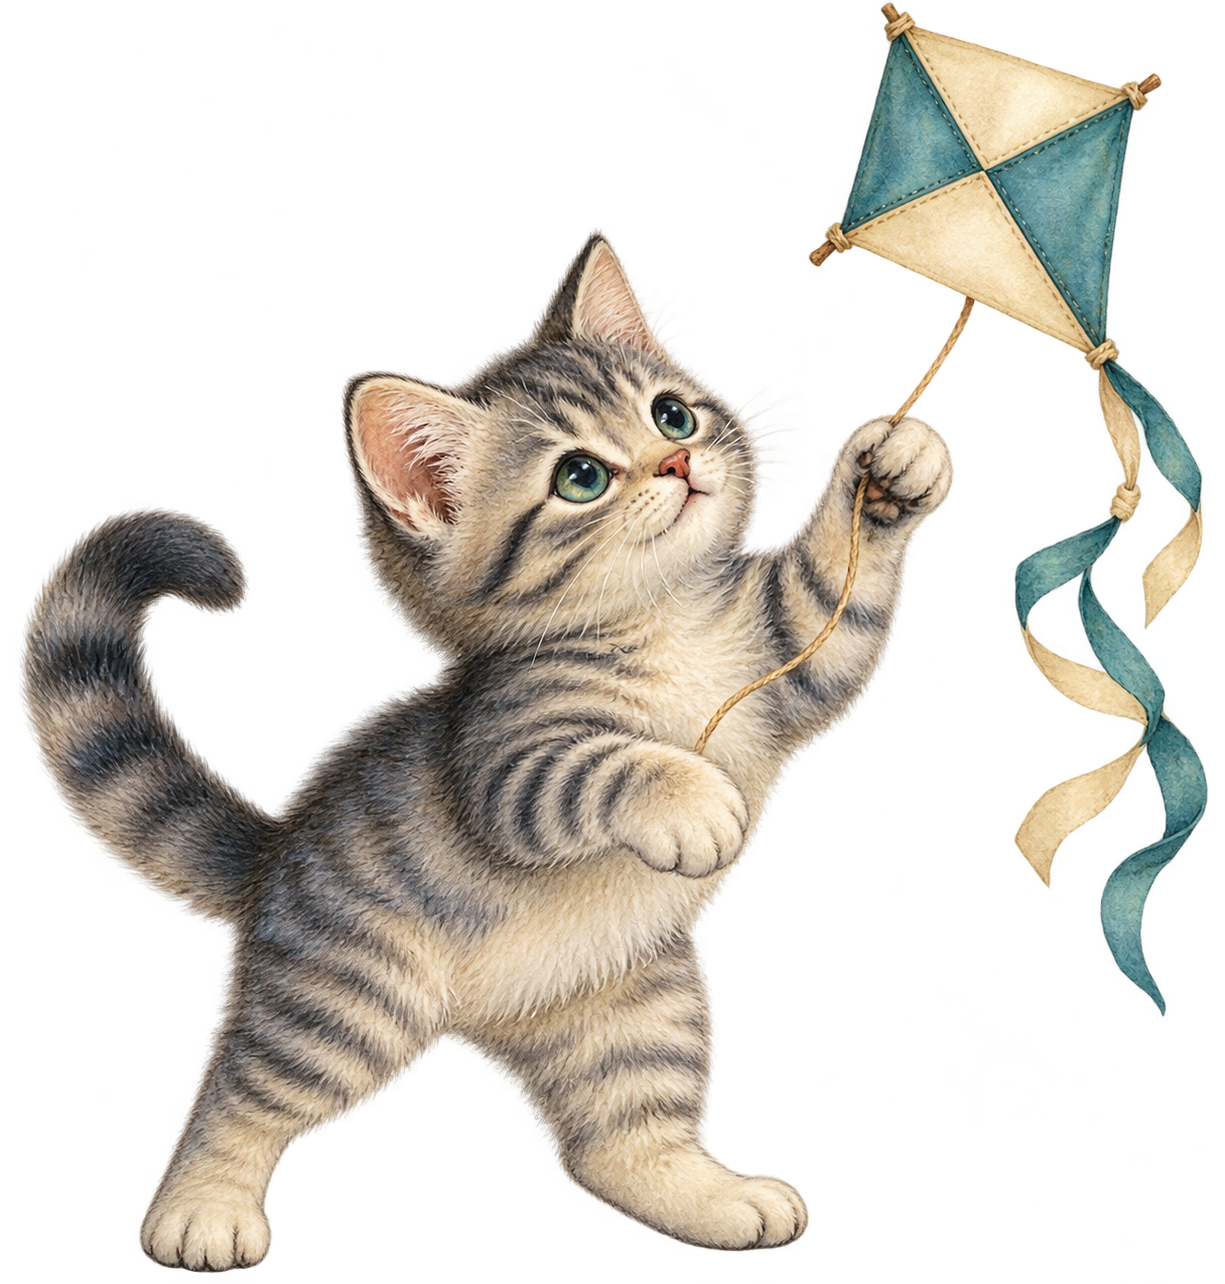
\includegraphics[width=54mm,height=58mm,keepaspectratio]{images/unique/art-138.png}
\label{catflow:138}
\end{wrapfigure}
Одинаковая формула со степенью точки объединяет несколько знакомых задач. Если точка снаружи, произведение двух отрезков секущей равно квадрату касательного отрезка. Если точка внутри, произведение расстояний до концов хорды одинаково для всех проходящих через неё хорд. Знак степени точки подсказывает, почему в этих двух ситуациях запись через положительные длины различается.
\par\WFclear\end{minipage}\end{lrbox}%
\ifdim\dimexpr\ht\CatFlowBox+\dp\CatFlowBox\relax<64mm\dp\CatFlowBox=\dimexpr64mm-\ht\CatFlowBox\relax\fi%
\noindent\usebox{\CatFlowBox}\par\addvspace{5pt}
\section{Тригонометрия треугольника}
\begin{theorem}[Косинусы и синусы; cosine and sine rules]
Для невырожденного треугольника
\[
c^2=a^2+b^2-2ab\cos C,\qquad
\frac a{\sin A}=\frac b{\sin B}=\frac c{\sin C}=2R,
\]
где \(R\) — радиус описанной окружности.
\end{theorem}
\begin{proof}Положим вершину \(C\) в начало координат, а одну сторону направим вдоль оси: концы сторон имеют координаты \((a,0)\) и \((b\cos C,b\sin C)\). Формула расстояния и \(\sin^2C+\cos^2C=1\) дают первую формулу, в том числе при тупом угле. Если \(A=\frac\pi2\), то сторона \(a\) — диаметр по свойству вписанного угла, и \(a=2R=2R\sin A\). В остальных случаях для второй формулы соединим конец стороны \(a\) с диаметрально противоположной точкой описанной окружности. Получится прямоугольный треугольник с гипотенузой \(2R\). Вписанный угол, опирающийся на ту же хорду, равен \(A\) либо \(\pi-A\); их синусы одинаковы. Поэтому \(a=2R\sin A\). Для остальных сторон рассуждение такое же. Свойство вписанного угла доказано выше.\end{proof}
\section{Площади и многоугольники}
\begin{definition}\term{Полупериметр} (\emph{semiperimeter}) треугольника равен \(p=\frac{a+b+c}2\). \par\term{Вписанная окружность} (\emph{incircle}) касается всех трёх сторон; её центр — пересечение внутренних биссектрис, радиус обозначают \(r\).\end{definition}
\begin{theorem}[Площади треугольника; Heron's formula]
\[
S=\frac12 ab\sin C=pr=\frac{abc}{4R}
=\sqrt{p(p-a)(p-b)(p-c)}.
\]
\end{theorem}
\begin{proof}Площадь равна половине произведения основания на высоту, откуда первая формула. Разбивая треугольник от центра вписанной окружности на три треугольника высоты \(r\), получаем \(S=\frac12(a+b+c)r\). Формула синусов даёт \(S=\frac12ab\frac c{2R}\). Наконец, по косинусам \(16S^2=4a^2b^2-(a^2+b^2-c^2)^2\). Разложение разности квадратов даёт \(16S^2=(a+b+c)(a+b-c)(a-b+c)(-a+b+c)\), то есть формулу Герона.\end{proof}
\begin{theorem}[Площадь параллелограмма и трапеции]
Параллелограмм с основанием \(a\) и высотой \(h\) имеет площадь \(ah\). Трапеция с основаниями \(a,b\) и высотой \(h\) имеет площадь \(\frac{a+b}2h\).
\end{theorem}
\begin{proof}Отрезанный прямоугольный треугольник параллелограмма переносится к противоположной стороне и дополняет фигуру до прямоугольника той же площади. Две одинаковые трапеции составляют параллелограмм с основанием \(a+b\) и высотой \(h\); делим его площадь пополам.\end{proof}
Для круга длина границы равна \(2\pi R\), площадь — \(\pi R^2\). Приближение правильными многоугольниками объясняет вторую формулу: площадь вписанного правильного многоугольника равна половине произведения его периметра на апофему, а в пределе эти величины стремятся к \(2\pi R\) и \(R\). Дуга угловой меры \(\theta\) радиан имеет длину \(R\theta\); соответствующий сектор — площадь \(\frac12R^2\theta\).
\begin{theorem}[Сумма внутренних углов выпуклого многоугольника]
Для выпуклого \(n\)-угольника сумма внутренних углов равна \((n-2)\pi\).
\end{theorem}
\par\addvspace{5pt}\begin{lrbox}{\CatFlowBox}\begin{minipage}[t]{\linewidth}
\setlength{\parskip}{5pt}\setlength{\columnsep}{4.5mm}\setlength{\intextsep}{0pt}
\begin{wrapfigure}[9]{l}{54mm}
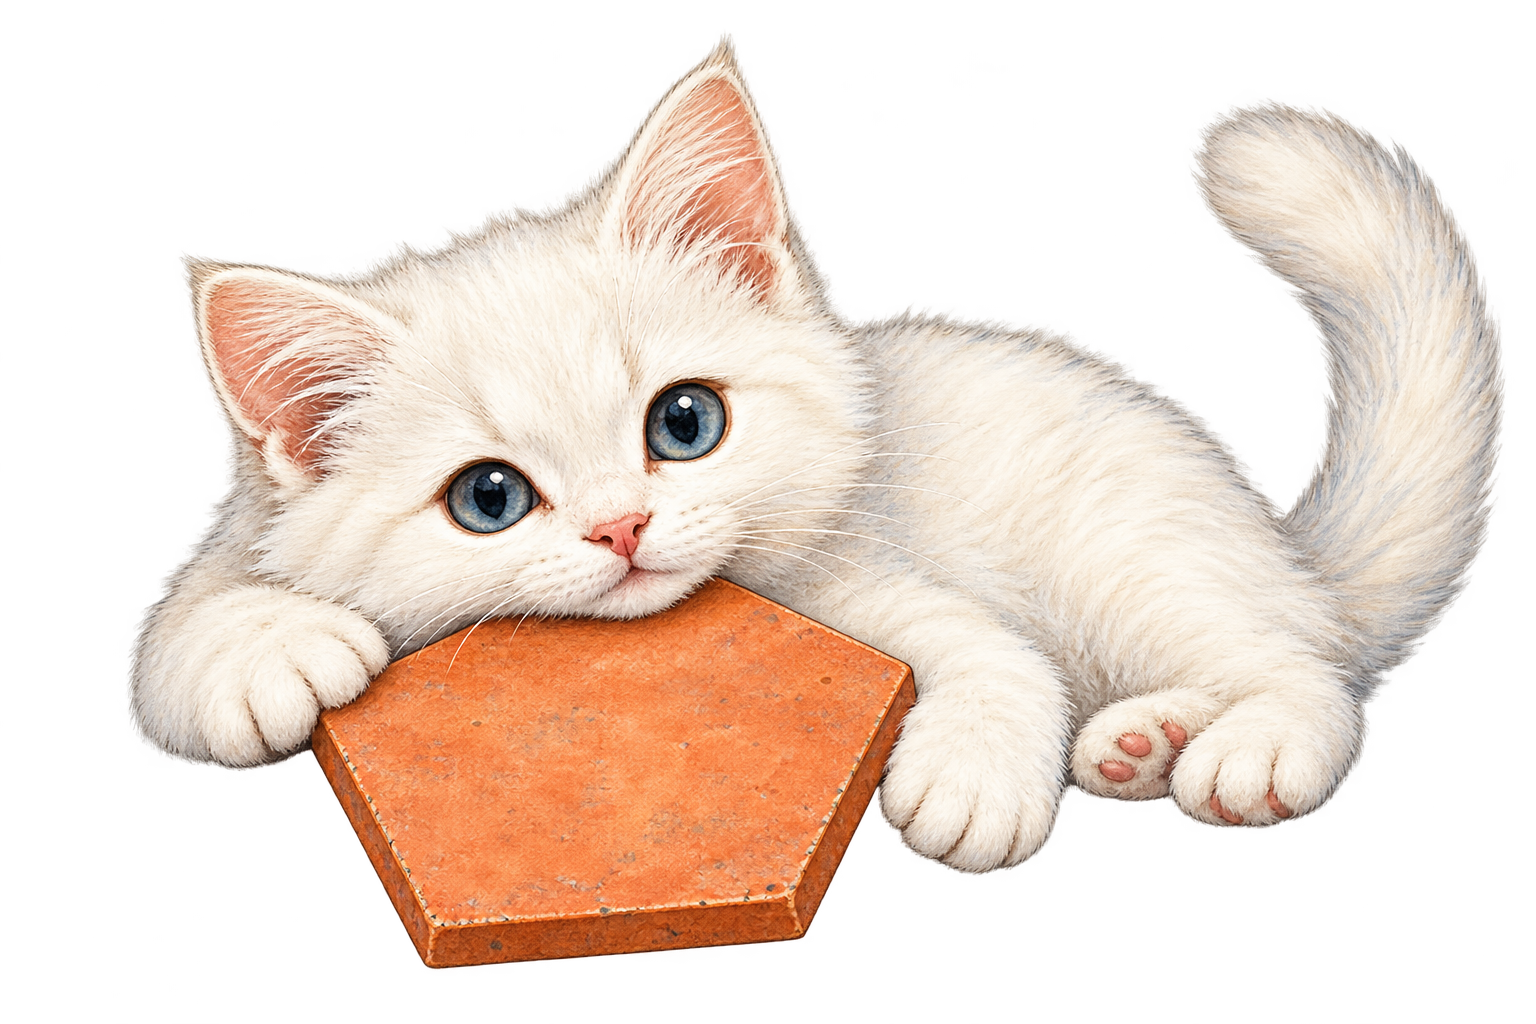
\includegraphics[width=54mm,height=58mm,keepaspectratio]{images/unique/art-139.png}
\label{catflow:139}
\end{wrapfigure}
\textit{Доказательство.} Диагонали из одной вершины разбивают его на \(n-2\) треугольника. Их внутренние углы вместе составляют все углы многоугольника.\hfill\(\blacksquare\)
\par\WFclear\end{minipage}\end{lrbox}%
\ifdim\dimexpr\ht\CatFlowBox+\dp\CatFlowBox\relax<64mm\dp\CatFlowBox=\dimexpr64mm-\ht\CatFlowBox\relax\fi%
\noindent\usebox{\CatFlowBox}\par\addvspace{5pt}


\par\noindent\begin{minipage}{\linewidth}\section*{Графики}
\begin{center}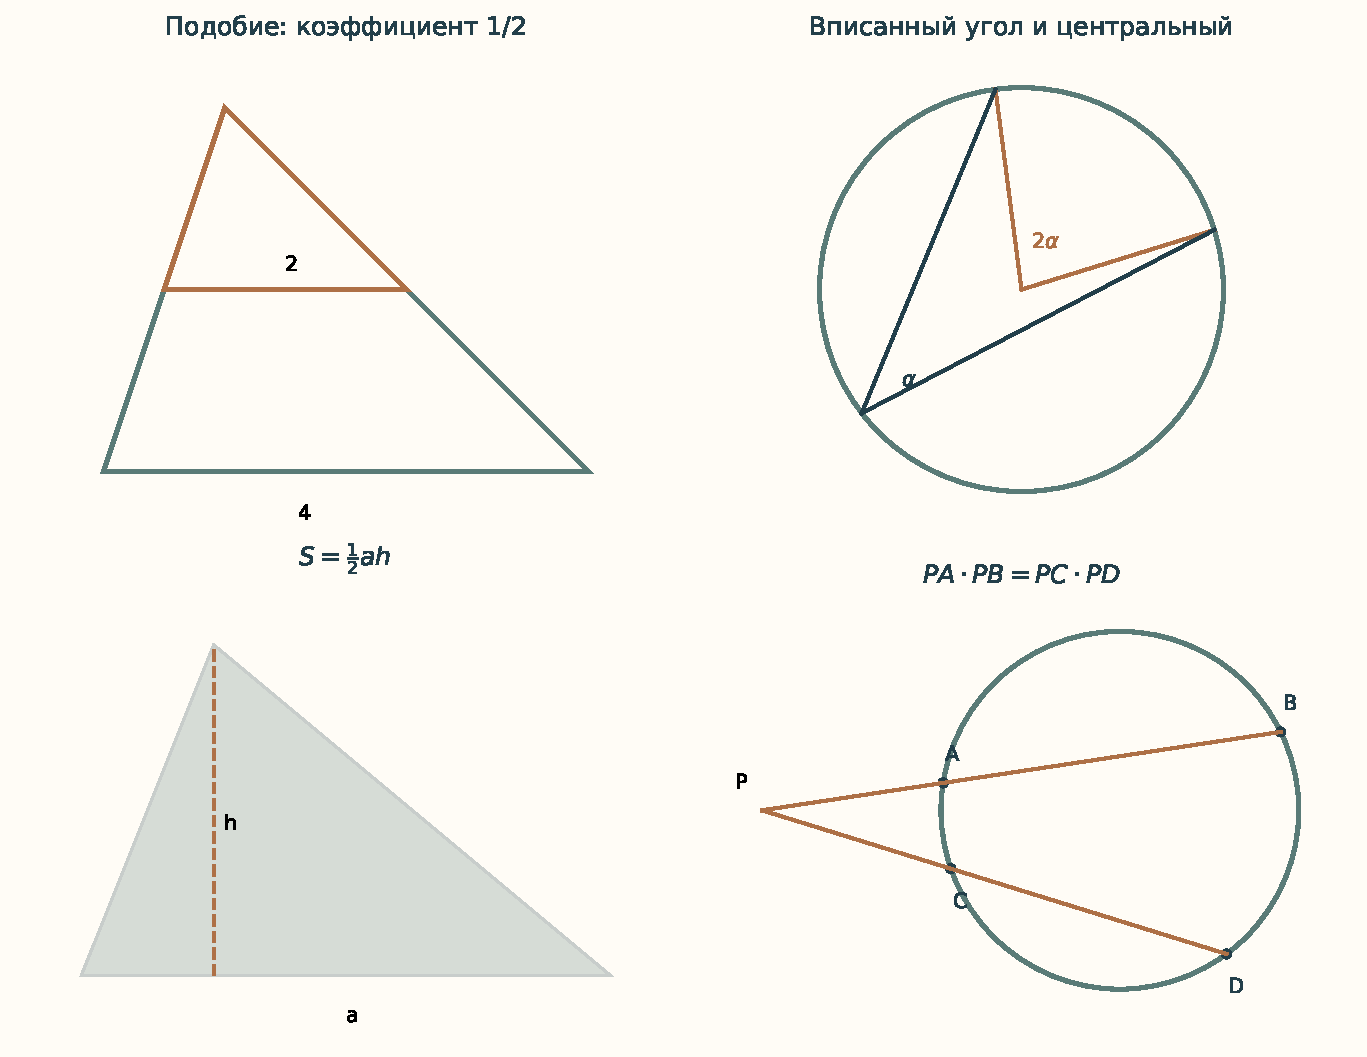
\includegraphics[width=\textwidth,height=.79\textheight,keepaspectratio]{images/atlas-plane-geometry.pdf}\par\small Подобие, окружность и площадь\end{center}\end{minipage}\par
\Needspace{7\baselineskip}\section*{Задачи}
\begingroup\setlength{\parskip}{2pt}
\noindent\begin{minipage}[t]{\linewidth}\textbf{28.1.} Два угла треугольника равны \(50^\circ\) и \(60^\circ\). Найди третий.\par\end{minipage}\par
\noindent\begin{minipage}[t]{\linewidth}\textbf{28.2.} Можно ли построить невырожденный треугольник со сторонами \(3,4,8\)?\par\end{minipage}\par
\noindent\begin{minipage}[t]{\linewidth}\textbf{28.3.} В равнобедренном треугольнике угол при вершине равен \(40^\circ\). Найди углы при основании.\par\end{minipage}\par
\noindent\begin{minipage}[t]{\linewidth}\textbf{28.4.} У прямоугольного треугольника катеты \(6,8\). Найди гипотенузу, площадь и радиусы вписанной и описанной окружностей.\par\end{minipage}\par
\noindent\begin{minipage}[t]{\linewidth}\textbf{28.5.} У подобных треугольников соответствующие стороны равны \(6\) и \(9\). Во сколько раз площадь второго больше площади первого?\par\end{minipage}\par
\par\addvspace{5pt}\begin{lrbox}{\CatFlowBox}\begin{minipage}[t]{\linewidth}
\setlength{\parskip}{5pt}\setlength{\columnsep}{4.5mm}\setlength{\intextsep}{0pt}
\begin{wrapfigure}[11]{r}{54mm}
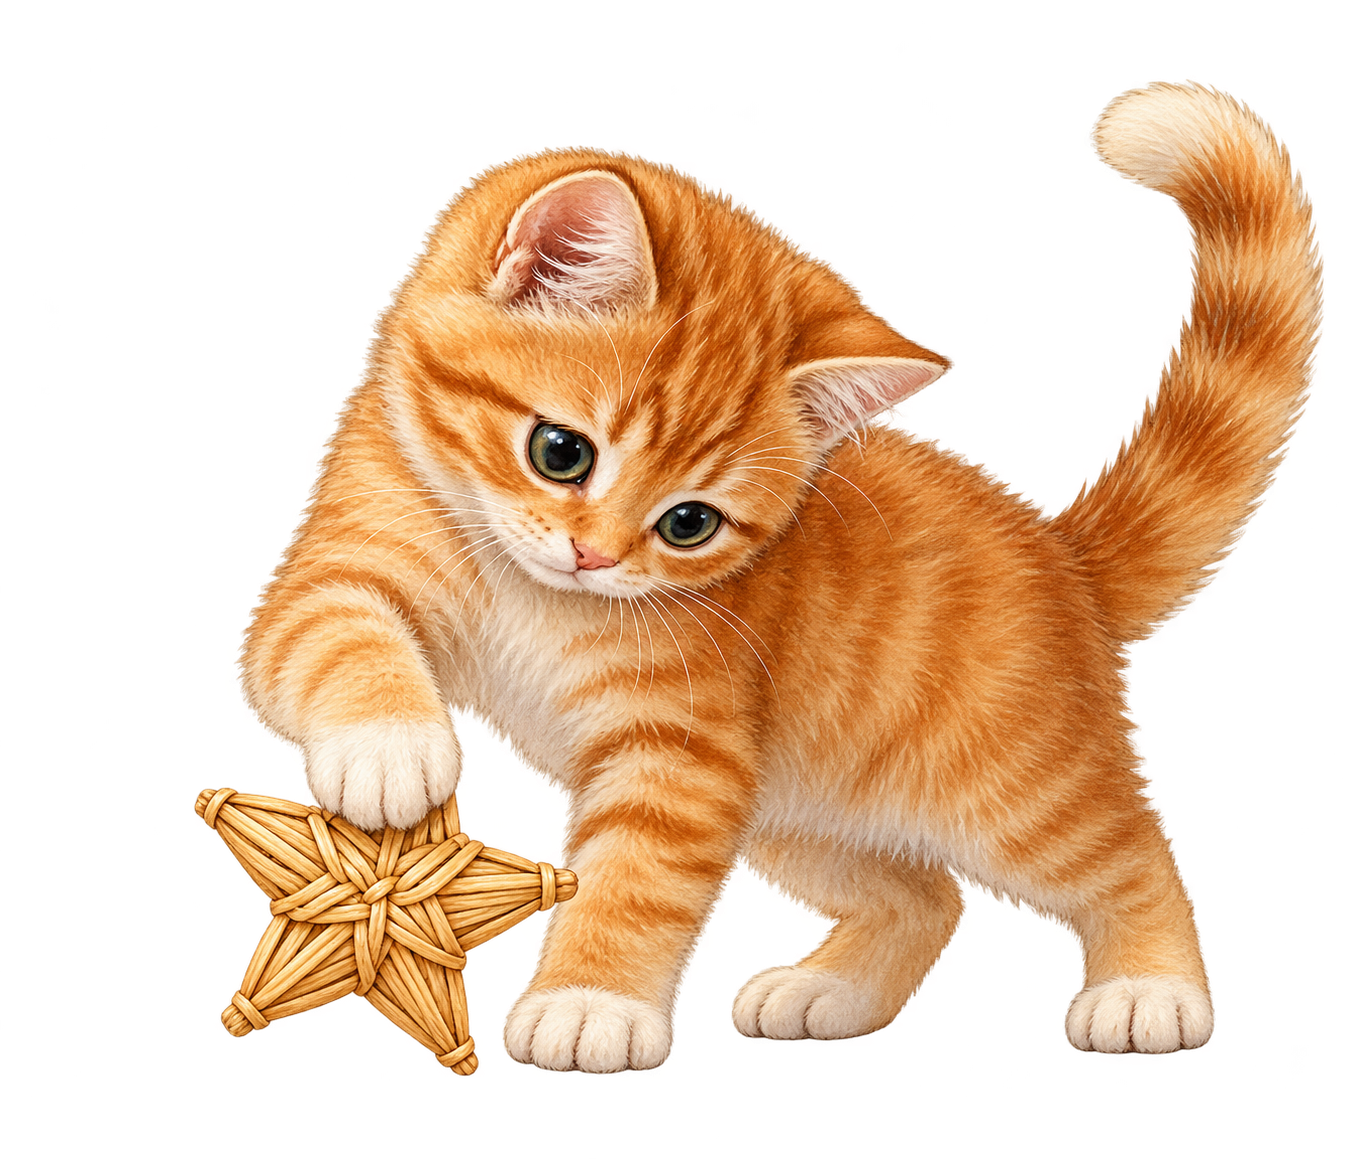
\includegraphics[width=54mm,height=58mm,keepaspectratio]{images/unique/art-140.png}
\label{catflow:140}
\end{wrapfigure}
\textbf{28.6.} В \(ABC\) проведено \(DE\parallel BC\), \(D\in AB\), \(E\in AC\). Даны \(AB=12\), \(AC=15\), \(AD=8\). Найди \(AE\) и отношение \(DE:BC\).\par

\textbf{28.7.} Две стороны треугольника равны \(5,7\), угол между ними \(60^\circ\). Найди третью сторону и площадь.\par

\textbf{28.8.} Сторона треугольника равна \(6\), противоположный угол \(30^\circ\). Найди радиус описанной окружности.\par

\textbf{28.9.} Для треугольника со сторонами \(13,14,15\) найди площадь, \(r\) и \(R\).\par
\par\WFclear\end{minipage}\end{lrbox}%
\ifdim\dimexpr\ht\CatFlowBox+\dp\CatFlowBox\relax<64mm\dp\CatFlowBox=\dimexpr64mm-\ht\CatFlowBox\relax\fi%
\noindent\usebox{\CatFlowBox}\par\addvspace{5pt}

\noindent\begin{minipage}[t]{\linewidth}\textbf{28.10.} У круга радиуса \(3\) выделен сектор угловой меры \(\dfrac{2\pi}3\). Найди длину его дуги и площадь.\par\end{minipage}\par
\noindent\begin{minipage}[t]{\linewidth}\textbf{28.11.} Вписанный угол равен \(35^\circ\). Найди угловую меру дуги, на которую он опирается, и соответствующий центральный угол.\par\end{minipage}\par
\noindent\begin{minipage}[t]{\linewidth}\textbf{28.12.} От точки на расстоянии \(13\) от центра окружности радиуса \(5\) проведена касательная. Найди длину касательного отрезка.\par\end{minipage}\par
\noindent\begin{minipage}[t]{\linewidth}\textbf{28.13.} Из внешней точки проведена секущая: расстояния до ближнего и дальнего пересечений равны \(4,9\). Найди длину касательного отрезка.\par\end{minipage}\par
\noindent\begin{minipage}[t]{\linewidth}\textbf{28.14.} Хорды пересекаются внутри окружности. На первой отрезки равны \(3,8\), на второй один отрезок равен \(4\). Найди другой.\par\end{minipage}\par
\noindent\begin{minipage}[t]{\linewidth}\textbf{28.15.} У правильного шестиугольника сторона \(2\). Найди периметр, радиус описанной окружности и площадь.\par\end{minipage}\par
\noindent\begin{minipage}[t]{\linewidth}\textbf{28.16.} Диагональ прямоугольника равна \(13\), сторона \(5\). Найди другую сторону и площадь.\par\end{minipage}\par
\noindent\begin{minipage}[t]{\linewidth}\textbf{28.17.} Найди площадь параллелограмма со сторонами \(6,4\) и углом \(30^\circ\) между ними.\par\end{minipage}\par
\noindent\begin{minipage}[t]{\linewidth}\textbf{28.18.} У трапеции основания \(6,10\) и высота \(3\). Найди площадь.\par\end{minipage}\par
\noindent\begin{minipage}[t]{\linewidth}\textbf{28.19.} Центр окружности \(O=(2,-1)\), радиус \(5\). Где находится точка \(P=(5,3)\): внутри, на границе или снаружи?\par\end{minipage}\par
\noindent\begin{minipage}[t]{\linewidth}\textbf{28.20.} Круглый пруд имеет радиус \(3\) м. От дорожной развилки до его центра \(5\) м. Найди длину прямого касательного участка от развилки до берега.\par\end{minipage}\par
\noindent\begin{minipage}[t]{\linewidth}\textbf{28.21.}\starmark{} Биссектриса угла \(A\) треугольника \(ABC\) встречает \(BC\) в \(D\). Докажи \(\dfrac{BD}{DC}=\dfrac{AB}{AC}\).\par\end{minipage}\par
\noindent\begin{minipage}[t]{\linewidth}\textbf{28.22.}\starmark{} Докажи, что медиана прямоугольного треугольника, проведённая к гипотенузе, равна половине гипотенузы.\par\end{minipage}\par
\noindent\begin{minipage}[t]{\linewidth}\textbf{28.23.}\starmark{} У прямоугольника периметр \(20\). Докажи, что площадь не больше \(25\), и укажи случай равенства.\par\end{minipage}\par
\noindent\begin{minipage}[t]{\linewidth}\textbf{28.24.}\starmark{} Среди треугольников с периметром \(12\) найди наибольшую площадь, используя формулу Герона и неравенство о среднем арифметическом и геометрическом.\par\end{minipage}\par
\par\Needspace{12\baselineskip}\section*{Олимпиадные задачи}
\noindent\begin{minipage}[t]{\linewidth}\textbf{28.25.}\starmark{} {\small\itshape\href{https://www.imo-official.org/assets/documents/problems/1961/1961_eng.pdf}{IMO, 1961, № 2}; перевод.}\par Для треугольника со сторонами \(a,b,c\) и площадью \(S\) докажи \(a^2+b^2+c^2\ge4\sqrt3\,S\). Когда достигается равенство?\par\end{minipage}\par
\noindent\begin{minipage}[t]{\linewidth}\textbf{28.26.}\starmark{} {\small\itshape\href{https://mmo.mccme.ru/books/mmo-35-57.pdf}{ММО, 1940, II тур, 7–8 классы, № 2}; редакция условия.}\par Равносторонний треугольник \(ABC\) вписан в окружность. Точка \(D\) лежит на меньшей дуге \(AB\). Докажи \(DC=DA+DB\).\par\end{minipage}\par
\endgroup
